\chapter{Numerics and Workflow}

    	 	\epigraph{On two occasions I have been asked, ``Pray, Mr. Babbage, if you put into the machine wrong figures, will the right answers come out?" ... I am not able rightly to apprehend the kind of confusion of ideas that could provoke such a question.}{Charles Babbage, Passages from the Life of a Philosopher}

Computational studies of Navier-Stokes, especially as a dynamical system, are difficult for many reasons, but most important among them is the high degree of complexity inherent in the numerical tools required to maintain efficiency. As mentioned earlier, the two major approaches towards simulating Navier-Stokes are modeling, where some assumptions are made to reduce the difficult of simulation, and direct numerical simulation (DNS), where no assumptions beyond those used to derive Navier-Stokes and set up the boundary conditions are used. DNS is naturally more accurate (since the physicality of some modeling assumptions can be suspect), but since it fully resolves Navier-Stokes, it is significantly more expensive than modeling, and methods that attempt to offset this extra cost tend to be extremely complex. For this reason, I use the open source library {\tt Channelflow}\rf{Gibson2014}, which has been essential in making any headway in this thesis. {\tt Channelflow} is a spectral DNS library, with additional utilities to find, parametrically continue, and analyze \ecs, which I will lay out in some detail below.
\section{The Spectral Method}
\subsection{The Residual}

Spectral methods are, like finite element methods, part of a larger class of numerical methods known as {\bf weighted residual methods}. In this class of methods, functions are approximated by a truncated series expansion, with the restriction that a quantity related to the residual be zero (instead of the residual itself). The quantity used for the spectral method is the scalar product 
\begin{equation}\label{eq:scalarProduct}
\scprod{u}{v}{w} = \int{a}{b}{uvw}{dx},
\end{equation}
where  $u(x),v(x)$ are some functions on the interval $[a,b]$, and $w(x)$ is a weighting function. If we then imagine some platonic function\footnote{That is, the function that is to be approximated} $u(x)$ that we attempt to approximate via a finite series expansion, so that
\begin{equation}\label{eq:seriesExpansion}
u_N(x) = \sum{k=0}{N}{\hat{u}_k \psi_k(x)},
\end{equation}
for some set of orthogonal basis functions $\psi_k(x)$, then the residual is given by
\begin{equation}
R_N = u(x)-u_N(x),
\end{equation} 
and for some differential equation
\begin{equation}
Du = f,
\end{equation}
where $D$ is some arbitrary differential operator and $f(x)$ is some arbitrary source function, the residual is defined
\begin{equation}
R_N = Du_N,
\end{equation}
as expected. While it may seem logical to require $R_N = 0$, this is not possible in general for finite $N$, so we instead require that for a set of test functions $\phi_i(x)$ and weighting function $w^*$, 
\begin{equation}\label{eq:SpectralZero}
\scprod{R_N}{\phi_i(x)}{w^*} = R_N(x_i) = 0,
\end{equation}
for some set of $x_i$. If $\phi_i(x) = \delta(x-x_i)$ and $w^* = 1$, then we have the colocation method, which forces the approximation to match the platonic function at a set of points. If $\phi_i(x) = \psi_i(x)$ and $w^* = w$, then we have the Galerkin method, which forces the mean residual to be zero. 

\subsection{Basis Functions}

In the spectral method, the basis functions are trigonometric functions. The advantage of trigonometric functions over polynomials is the rapid convergence of the series coefficients -- the Fourier coefficients converge exponentially fast, so we can achieve extremely high accuracy with a lower number of modes\rf{Peyret2002}.\footnote{Spectral methods are inappropriate when the boundary geometry is highly complex, as is the case in the majority of industrial applications, where more general finite element methods are used.} {\tt Channelflow} uses Fourier series in the streamwise-spanwise directions, where the basis functions and spectral projection are given by 
\begin{align}
F_k(x) = \exp{ikx}\\
u_K(x) = \sum{k=-K}{K}\hat{u}_k\exp{ikx},
\end{align}
and Chebyshev polynomials of the first kind in the wall-normal direction, where the basis functions and spectral projection are given by
\begin{align}
T_k(x) = \cos{k\arccos{x}}\\
u_N(x) = \sum{k=0}{(2k-1)/2}\hat{\mathfrak{u}}_kT_k(x).
\end{align}
\par The Fourier series expansion is particularly nice since the derivative $\partial_x F_k(x) = ikF(x)$ is especially easy to calculate, as are the Fourier coefficients by virtue of the Fast Fourier Transform, implemented in the Fastest Fourier Transform in the West (FFTW)\rf{Frigo1998}.\\

For Chebyshev polynomials, the derivative is slightly more complicated, since 
\begin{equation}
\partial_x T_k(x) = 2k\sum{n=0}{K}{\frac{1}{c_{k-1-2n}} T_{k-1-2n}(x)},
\end{equation}
where $c_k = 1$ if $k=1$ and $2$ if $k > 1$. Since the derivative of a single Chebyshev term becomes a sum of Chebyshev terms, the derivative of the Chebyshev representation of a function 
\begin{align}
\partial_x \sum{k=0}{N}\hat{\mathfrak{u}}_kT_k(x) &= \sum{k=0}{N}\hat{\mathfrak{u}}_k^{(1)}T_k(x),\\
\hat{\mathfrak{u}}_k^{(1)} &= \frac{2}{c_k}\sum{\substack{p = k+1\\(p+k) \mathrm{~odd}}}{N} p \hat{\mathfrak{u}}_p, \hspace{0.25cm} k \neq N,\\
\hat{u}^{(1)}_N &= 0.
\end{align}
As with the Fourier decomposition, however, Chebyshev coefficients can be calculated by a discrete cosine transform\rf{Halcrow2008}, which is a special case of the discrete Fourier transform, and is thus also computed by FFTW. 

While Fourier expansions are the easiest to deal with, they are best used on periodic boundaries, since the imposition of aperiodic boundary conditions on a Fourier series expansion can lead to Gibbs oscillations that can make the simulation aphysical\rf{Peyret2002}. For this reason, the velocity field is expanded as a Fourier series in the plane, and as a Chebyshev polynomial in the wall-normal direction. The velocity field is then represented as 
\begin{equation}
\Vector{u}_{KJL}(x,y,z) = \sum{k=-K}{K}{\hat{u}_k(x)\exp{ikx}}\sum{j=-J}{J}{\hat{u}_j(z)\exp{ijz}}\sum{l=0}{L}{\hat{\mathfrak{u}}_l(y)T_l(y)}.
\end{equation}

\subsection{Spatio-Temporal Discretization} 

Under the (Galerkin) spectral approximation 
\begin{equation}
\Vector{u}(x,y,z) = \Vector{U}_{KJL}(x,y,z),
\end{equation}
the partial differential equation
\begin{equation}
\pder{1}{\Vector{u}}{t} = f_T(\Vector{u}),
\end{equation}
becomes an ordinary differential equation (ODE)
\begin{equation}
\der{1}{\Vector{U_{KJL}}}{t} = F_T(\Vector{U}_{KJL}), 
\end{equation}
where $f_T(\Vector{u})$ is the forward time evolution of the Navier-Stokes equation, and $F_T(\Vector{U}_{KJL})$ is its spectral approximation via \refeq{eq:SpectralZero}. The temporal ODE can be solved in any number of ways -- {\tt Channelflow} allows the user to choose from several implicit-explicit methods, where the implicit : Crank-Nicolson Forward Euler, Crank-Nicolson Adams-Bashforth, Spalart-Moser Runge-Kutta and Semi-implicit Backwards Differentiation of orders 1 to 4. The order 3 Semi-implicit Backwards Differentiation (SBDF3) was chosen by default, and no reason to change this was anticipated, since SBDF3 is known to have a relatively large time step and low error for large \ReN\rf{Ascher1995}.

\section{Newton-Krylov-Hookstep Method}

In order to find \ecs\, it is necessary to solve the equation
\begin{equation}\label{eq:NRResidual}
\Vector{u} - \sigma f_T(\Vector{u}) = R_T(\Vector{u}) = 0,
\end{equation}
which is easiest tackled by root-finding algorithms. The root finding method used by {\tt Channelflow} is based on Newton's method, with some additional refinements. \\
\subsection{Newton's Method}
The principle behind Newton's method is as follows: Suppose we have $f(x)$ be a smooth and differentiable function, and an initial, `good' guess\footnote{How good a guess needs to be is highly dependent on the problem. Through this thesis, an initial condition that gave $R_T(\Vector{u}) < 0.001$ was considered a sufficiently good guess.}  $x_0$ for the root of $f$. Then we can find a better guess for the root of $f$ by finding the root of the tangent line at $f(x_0)$ (\refFig{fig:Newton}). Mathematically, 
\begin{align}
f(x_n) + f'(x_n)\paren{x_{n+1} - x_n} = 0,\label{eq:NRS1D}\\ 
x_{n+1} = x_n - \frac{f(x_n)}{f'(x_n)}.\label{eq:NR1D}
\end{align}
In higher dimensions, \refeqs{eq:NRS1D}{eq:NR1D} are replaced by the matrix equations
\begin{align}
\Vector{f}(\Vector{x}_n) + \mathbb{J}_{f,\Vector{x_n}}(\Vector{x}_{n+1} - \Vector{x}_n) = 0,\label{eq:NRSND}\\
\Vector{x}_{n+1} = \Vector{x}_n - \mathbb{J}_{f,\Vector{x}_n}^{-1}\Vector{f}(\Vector{x}_n)
\end{align}
where $\mathbb{J}_{f,\Vector{x_n}}$ is the Jacobian of the Navier-Stokes equation at $\Vector{x}_n$.\\
 
Newton's method is extremely fast and converges quadratically on the root\rf{Press2007}, but is not guaranteed to do so - a simple example is if the $n$-th guess is at (or very close to) a local minimum, in which case the adjustment term of \refeq{eq:NR1D} will explode, taking us very far away from the initial, good guess. As a result, 
\begin{figure}[h]
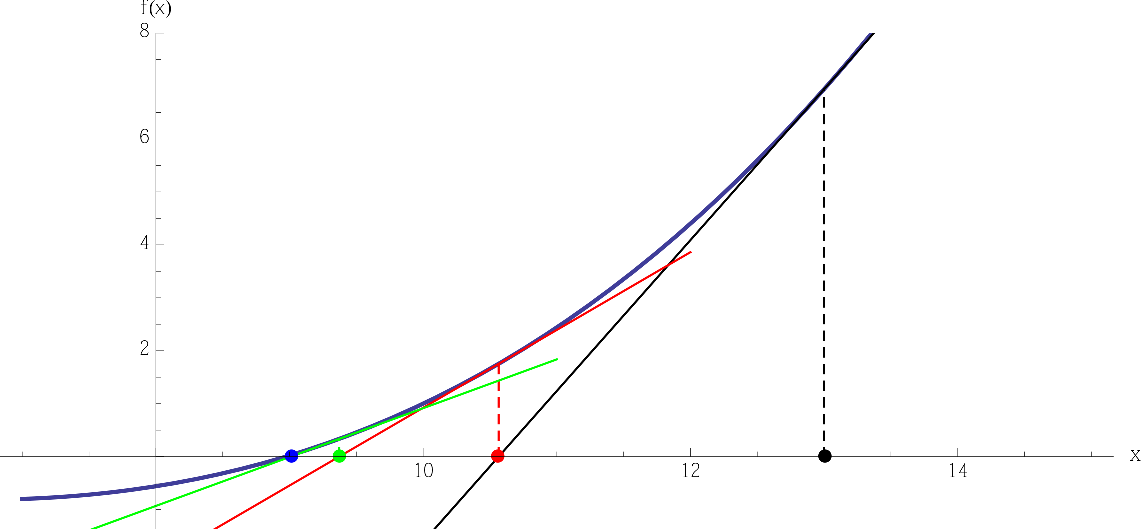
\includegraphics[width=\textwidth]{NRMethod}
\caption{A demonstration of Newton's method in 1D on a simple function with the root at $x_r \approx 8.98$. Starting at $x_0$ = 13, the method converges to $10^{-4}$ in just three steps.}\label{fig:Newton}
\end{figure}  


